\chapter{Semi-passive knee design} % (fold)
\label{appendix:knee_optimization}

\section{Introduction} % (fold)

We performed a parametric optimization both on the position of the spring ties ($M_T$ and $M_L$) and on its characteristic ($K$, $L_0$, $D_i$, $F_{max}$, $L_{max}$) (see Fig.~\ref{fig:knee_conception}) to try to match the mentioned criterion above. These criterion are modelled as condition on the resultant torque:

\begin{itemize}
    \item $C(\theta=0) < -0.4$: Locking of the knee, where $0.4 N.m$ is the necessary torque to keep the leg straight.
    \item $C(\theta=25 \textsuperscript{o} ) = 0$: Transition between the two behaviors
    \item $C > 0$ if $\theta > 25 deg$: Helps the motor to lift the leg.
    \item $ max(\abs{C(\theta)}) < \frac{C_{MX-28}}{2}$: The actuator $MX-28$ should always be powerful enough to control the joint motion.
\end{itemize}

\begin{figure}[ht]
    \centering
    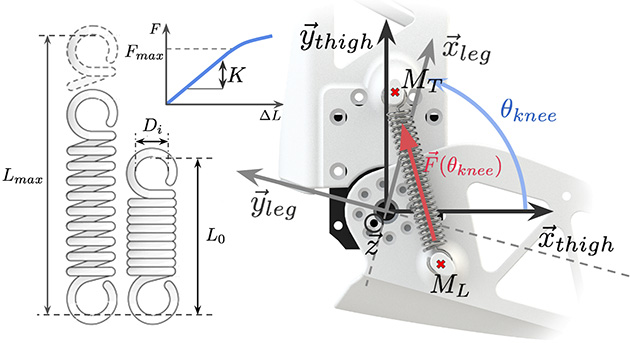
\includegraphics[width=0.9\linewidth]{knee_spring.jpg}
    \caption{Spring parameters to optimize}
    \label{fig:knee_conception}
\end{figure}


The resultant torque $C$ generated by springs in function of the knee flexion $\theta$  ($n_{spring} = 2$) is computed as follow:

\begin{equation}
    C(\theta) = n_{spring} \cdot \overrightarrow{OM_L}{\rvert}_{R_{thigh}} \wedge \overrightarrow{F}(\theta) \cdot \overrightarrow{z}
\end{equation}

with:

\begin{equation}
    \norm{ F(\theta)} = K \cdot \left ( L(\theta) - L_0\right )
\end{equation}

\begin{equation}
    L(\theta) = \quad \norm{ \overrightarrow{M_T M_L}{\rvert}_{R_{thigh}}}\qquad
\end{equation}

\begin{equation}
    \overrightarrow{OM_L}{\rvert}_{R_{thigh}}  = \overrightarrow{OM_L}{\rvert}_{R_{leg}}  \cdot
    \begin{bmatrix}
        cos(\theta) & -sin(\theta) & 0 \\
        sin(\theta) & cos(\theta) & 0 \\
        0 & 0 & 1\\
    \end{bmatrix}
\end{equation}



We use an iterative selection on these criteria to determine the appropriate characteristics for the spring.

\section{Minimizing stresses on the structure} % (fold)
\label{par:minimize_stresses_on_the_structure}

The length of the lever arm is constrained by the dimensions of the legs, resulting in an increase of the force generated by the spring to produce the desired torque on the knee.

By maximizing the following criterion with the constraint $C(\theta=25 \textsuperscript{o} ) = 0$:
\begin{equation}
     c_1 = \frac{C_{max}}{F_{max}^2}
\end{equation}

We were able to determine the ties’ specific location ($M_T$ and $M_L$), for both minimizing mechanical stress and changing the torque direction for $\theta = 25\textsuperscript{o}$,


\begin{equation}
    M_T={\left \{2,39,0 \right \}_R}_{thigh}
    \qquad
    M_L = {\left \{-12,23,0 \right \}_R}_{leg}
\end{equation}

and constraints concerning the springs characteristics:
\begin{equation}
    L_{min} < 42.6 mm
    \qquad
    L_{max} > 65.12 mm
\end{equation}


\section{Ties strength} % (fold)
\label{par:ties_strength}

We calculated the minimum diameter of the ties required to withstand the constraints imposed by the spring with a beam theory model:
\begin{equation}
    D_{min}= \sqrt[3]{ \frac{32 \times  C_s \times F_{max} \times l_{tie}}{2 \pi \times \sigma_{MaxPolyamide}} }
\end{equation}
By considering Poppy's parameters and a coefficient of safety $C_s = 5$, we have found that the spring must respect the criterion $D_{min} > 6.5 mm$.

\section{Obtained behavior} % (fold)
\label{sub:obtained_behavior}

Considering the desired spring behavior and geometrical conditions, an automatic selection out of 720 different springs\footnote{pre-selection of springs in the vanel.com catalog} was performed. Only 5 springs satisfied all criteria. For the Poppy platform we chose a spring with the following characteristics: $\{ D_i=9.6mm$, $L_0=42mm$, $K=1620N.m^{-1}$, $F_{max}=81.7 N$, $L_{max}=72.8 mm \}$ inducing a resultant behavior shown in Fig.~\ref{fig:knee_feature}. As we can see, even if the torque applied by the spring is quite low ($C_{max} = 0.74 N.m$), the force subjected to spring ties is up to $40N$. The shape of the ties has been optimized using FEA (Finite Element Analysis) in order to handle the stress.

\begin{figure}[ht]
    \centering
    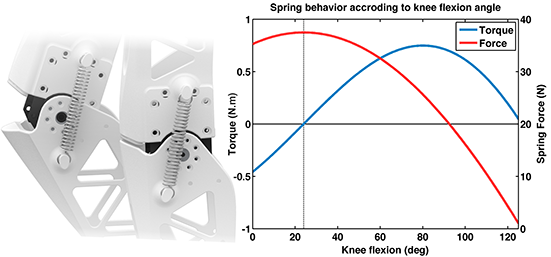
\includegraphics[width=0.95\linewidth]{torque_knee.png}
    \caption{Theoretical semi-passive mechanism behavior. The blue line corresponds to the torque applied by the springs on the leg according to the flexion angle of the knee. The red line corresponds to the force that the springs applied on ties.}
    \label{fig:knee_feature}
\end{figure}
